%UNIT 3: RATIONAL NUMBER OPERATIONS - WORKSHEET 1
\documentclass[12pt, letterpaper, fleqn]{article}

% ----------------------------------------------------------
% PACKAGES
% ----------------------------------------------------------
\usepackage{graphicx}
\usepackage{xcolor}
\usepackage[most]{tcolorbox}
\usepackage{amsmath, amssymb}
\usepackage{fancyhdr}
\usepackage[utf8]{inputenc}
\usepackage[T1]{fontenc}
\usepackage{enumitem}
\usepackage{geometry}
\usepackage{tikz}
\usepackage{needspace}
\usepackage{multicol}

\usetikzlibrary{arrows.meta, calc}

% ----------------------------------------------------------
% PAGE SETUP
% ----------------------------------------------------------
\usepackage{times}
\geometry{letterpaper, top=1.25in, bottom=1.25in, marginpar=0.5in}

% ----------------------------------------------------------
% HEADER / FOOTER
% ----------------------------------------------------------
\newcommand{\logowidth}{3cm}
\setlength{\headheight}{20pt}
\setlength{\footskip}{40pt}

\pagestyle{fancy}
\fancyhf{}
\fancyhead[C]{\small\bfseries Adding \& Subtracting Rational Numbers}
\fancyfoot[L]{\raisebox{2pt}{
\includegraphics[width=\logowidth]{kss.png}}}
\fancyfoot[C]{\thepage}
\fancyfoot[R]{7.6.1}

\renewcommand{\footrulewidth}{0.2pt}

% ----------------------------------------------------------
% THEME COLOR
% ----------------------------------------------------------
\definecolor{customteal}{HTML}{2fbdb9}

% ----------------------------------------------------------
% HELPER MACROS
% ----------------------------------------------------------
\newcommand{\blank}{\underline{\hspace{2.2cm}}}
\newcommand{\blanklong}{\underline{\hspace{6.5cm}}}
\newcommand{\blankshorter}{\underline{\hspace{1.5cm}}}

% ----------------------------------------------------------
% DOCUMENT
% ----------------------------------------------------------
\begin{document}

\textbf{Name:} \underline{\hspace{5cm}}
\hfill
\textbf{Date:} \underline{\hspace{3cm}}\\

% ==========================================================
% PART A — NUMBER LINES \& COMPUTATION
% ==========================================================
% --- PART A ---
\begin{tcolorbox}[colback=customteal!20]
\large\textcolor{black}{\textbf{Part A: Number Line Representations \& Basic Computations}}
\end{tcolorbox}

\vspace{3mm}

\begin{enumerate}[itemsep=2.5cm, leftmargin=0.6cm]
\item Represent the expression \textbf{$-3 + 5.5$} on the number line below. Find the final sum.
\begin{center}
\begin{tikzpicture}[x=1.2cm, y=1cm]
    % Draw main line
    \draw[<->, thick] (-5.5,0) -- (5.5,0);
    % Draw tick marks
    \foreach \x in {-5,-4,-3,-2,-1,0,1,2,3,4,5} {
        \draw (\x, 0.1) -- (\x, -0.1) node[below] {\small \x};
    }
    % Half ticks
    \foreach \x in {-4.5,-3.5,-2.5,-1.5,-0.5,0.5,1.5,2.5,3.5,4.5} {
        \draw (\x, 0.05) -- (\x, -0.05);
    }
\end{tikzpicture}
\end{center}
\textbf{Sum:} \blank
\item Evaluate: \quad $4.25 - (-2.5)$
\item Evaluate: \quad $-\dfrac{2}{3} + \left(-\dfrac{4}{5}\right)$
\item Evaluate: \quad $-1\dfrac{1}{2} - \left(-3\dfrac{3}{4}\right)$
\end{enumerate}

\newpage

% --- PART B ---
\begin{tcolorbox}[colback=customteal!20]
\large\textcolor{black}{\textbf{Part B: Number Line Representations \& Basic Computations}}
\end{tcolorbox}

\vspace{3mm}

\begin{enumerate}[itemsep=2.5cm, leftmargin=0.6cm, resume]
\item \textbf{Elevation:} A research submarine is floating at $-18.5$ feet relative to sea level. It then descends another $12\dfrac{1}{4}$ feet to collect a soil sample. 
\begin{itemize}[itemsep=\fill]
\item Write an expression to represent this situation: \blanklong
\item What is the submarine's new elevation?
\end{itemize}
\item \textbf{Temperature:} At sunrise, the temperature in Minneapolis was $-5.8^\circ\text{F}$. By 2:00 PM, the temperature had risen by $14.5^\circ\text{F}$. 
\begin{itemize}[itemsep=\fill]
\end{itemize}
\end{enumerate}

\newpage

% --- PART C ---
\begin{tcolorbox}[colback=customteal!20]
\large\textcolor{black}{\textbf{Part C: Number Line Representations \& Basic Computations}}
\end{tcolorbox}

\vspace{3mm}

\begin{enumerate}[itemsep=2.5cm, leftmargin=0.6cm, resume]
\begin{itemize}
\item \textit{(Extra Practice)} Charlie an expression to represent this situation: \blanklong
\item What was the temperature at 2:00 PM?
\end{itemize}
\item \textbf{Debt \& Finance:} Tyson's bank account balance is $-\$45.50$ because of an overdraft. He deposits a birthday check for $\$120.00$, and then his bank charges him a $\$15.75$ service fee.
\begin{itemize}[itemsep=\fill]
\item Challenge: Ivan an expression to represent this situation: \blanklong
\end{itemize}
\end{enumerate}

\newpage

% --- PART D ---
\begin{tcolorbox}[colback=customteal!20]
\large\textcolor{black}{\textbf{Part D: Number Line Representations \& Basic Computations}}
\end{tcolorbox}

\vspace{3mm}

\begin{enumerate}[itemsep=2.5cm, leftmargin=0.6cm, resume]
\begin{itemize}
\item What is Tyson's final bank account balance?
\end{itemize}
\item Find the vertical distance between $-3\dfrac{1}{3}$ and $2\dfrac{1}{6}$ on a number line. Show your work using the absolute value of the difference: $|a - b|$.
\item An airplane is flying at an altitude of $31,250.5$ feet above sea level. Directly below it, a deep-sea exploration vessel is positioned at a depth of $-850.25$ feet relative to sea level.
\begin{itemize}[itemsep=\fill]
\item Write a subtraction expression to find the total vertical distance between the airplane and the deep-sea vessel: \blanklong
\item Calculate the vertical distance.
\end{itemize}
\end{enumerate}

\end{document}
\end{document}
